% Options for packages loaded elsewhere
\PassOptionsToPackage{unicode}{hyperref}
\PassOptionsToPackage{hyphens}{url}
%
\documentclass[
  ignorenonframetext,
]{beamer}
\usepackage{pgfpages}
\setbeamertemplate{caption}[numbered]
\setbeamertemplate{caption label separator}{: }
\setbeamercolor{caption name}{fg=normal text.fg}
\beamertemplatenavigationsymbolsempty
% Prevent slide breaks in the middle of a paragraph
\widowpenalties 1 10000
\raggedbottom
\setbeamertemplate{part page}{
  \centering
  \begin{beamercolorbox}[sep=16pt,center]{part title}
    \usebeamerfont{part title}\insertpart\par
  \end{beamercolorbox}
}
\setbeamertemplate{section page}{
  \centering
  \begin{beamercolorbox}[sep=12pt,center]{part title}
    \usebeamerfont{section title}\insertsection\par
  \end{beamercolorbox}
}
\setbeamertemplate{subsection page}{
  \centering
  \begin{beamercolorbox}[sep=8pt,center]{part title}
    \usebeamerfont{subsection title}\insertsubsection\par
  \end{beamercolorbox}
}
\AtBeginPart{
  \frame{\partpage}
}
\AtBeginSection{
  \ifbibliography
  \else
    \frame{\sectionpage}
  \fi
}
\AtBeginSubsection{
  \frame{\subsectionpage}
}
\usepackage{amsmath,amssymb}
\usepackage{iftex}
\ifPDFTeX
  \usepackage[T1]{fontenc}
  \usepackage[utf8]{inputenc}
  \usepackage{textcomp} % provide euro and other symbols
\else % if luatex or xetex
  \usepackage{unicode-math} % this also loads fontspec
  \defaultfontfeatures{Scale=MatchLowercase}
  \defaultfontfeatures[\rmfamily]{Ligatures=TeX,Scale=1}
\fi
\usepackage{lmodern}
\ifPDFTeX\else
  % xetex/luatex font selection
\fi
% Use upquote if available, for straight quotes in verbatim environments
\IfFileExists{upquote.sty}{\usepackage{upquote}}{}
\IfFileExists{microtype.sty}{% use microtype if available
  \usepackage[]{microtype}
  \UseMicrotypeSet[protrusion]{basicmath} % disable protrusion for tt fonts
}{}
\makeatletter
\@ifundefined{KOMAClassName}{% if non-KOMA class
  \IfFileExists{parskip.sty}{%
    \usepackage{parskip}
  }{% else
    \setlength{\parindent}{0pt}
    \setlength{\parskip}{6pt plus 2pt minus 1pt}}
}{% if KOMA class
  \KOMAoptions{parskip=half}}
\makeatother
\usepackage{xcolor}
\newif\ifbibliography
\usepackage{graphicx}
\makeatletter
\def\maxwidth{\ifdim\Gin@nat@width>\linewidth\linewidth\else\Gin@nat@width\fi}
\def\maxheight{\ifdim\Gin@nat@height>\textheight\textheight\else\Gin@nat@height\fi}
\makeatother
% Scale images if necessary, so that they will not overflow the page
% margins by default, and it is still possible to overwrite the defaults
% using explicit options in \includegraphics[width, height, ...]{}
\setkeys{Gin}{width=\maxwidth,height=\maxheight,keepaspectratio}
% Set default figure placement to htbp
\makeatletter
\def\fps@figure{htbp}
\makeatother
\usepackage{svg}
\setlength{\emergencystretch}{3em} % prevent overfull lines
\providecommand{\tightlist}{%
  \setlength{\itemsep}{0pt}\setlength{\parskip}{0pt}}
\setcounter{secnumdepth}{-\maxdimen} % remove section numbering
\newlength{\cslhangindent}
\setlength{\cslhangindent}{1.5em}
\newlength{\csllabelwidth}
\setlength{\csllabelwidth}{3em}
\newlength{\cslentryspacingunit} % times entry-spacing
\setlength{\cslentryspacingunit}{\parskip}
\newenvironment{CSLReferences}[2] % #1 hanging-ident, #2 entry spacing
 {% don't indent paragraphs
  \setlength{\parindent}{0pt}
  % turn on hanging indent if param 1 is 1
  \ifodd #1
  \let\oldpar\par
  \def\par{\hangindent=\cslhangindent\oldpar}
  \fi
  % set entry spacing
  \setlength{\parskip}{#2\cslentryspacingunit}
 }%
 {}
\usepackage{calc}
\newcommand{\CSLBlock}[1]{#1\hfill\break}
\newcommand{\CSLLeftMargin}[1]{\parbox[t]{\csllabelwidth}{#1}}
\newcommand{\CSLRightInline}[1]{\parbox[t]{\linewidth - \csllabelwidth}{#1}\break}
\newcommand{\CSLIndent}[1]{\hspace{\cslhangindent}#1}
\ifLuaTeX
  \usepackage{selnolig}  % disable illegal ligatures
\fi
\IfFileExists{bookmark.sty}{\usepackage{bookmark}}{\usepackage{hyperref}}
\IfFileExists{xurl.sty}{\usepackage{xurl}}{} % add URL line breaks if available
\urlstyle{same}
\hypersetup{
  pdftitle={Octree Frontend for Enzo-E in YT},
  pdfauthor={Bolun Thompson REU FoDoMMaT Visiting Scholar ; Matthew Turk Assistant Professor at the School of Information Sciences },
  hidelinks,
  pdfcreator={LaTeX via pandoc}}

\title{Octree Frontend for Enzo-E in YT}
\author{Bolun Thompson\\
REU FoDoMMaT Visiting Scholar\\ \and Matthew Turk\\
Assistant Professor at the School of Information Sciences\\}
\date{July 6th, 2023}

\begin{document}
\frame{\titlepage}

\begin{frame}{Volumetric Simulations}
\protect\hypertarget{volumetric-simulations}{}
\begin{itemize}
\tightlist
\item
  Formation of stars and galaxies
\item
  Nuclear reactor mechanics
\end{itemize}
\end{frame}

\begin{frame}{Why?}
\protect\hypertarget{why}{}
Connects theories with data
\end{frame}

\begin{frame}{What}
\protect\hypertarget{what}{}
\begin{itemize}
\tightlist
\item
  Enzo: \textbf{Adaptive Mesh Refinement} (AMR) astrophysical simulation
  code {[}1{]}

  \begin{itemize}
  \tightlist
  \item
    Multi-purpose
  \end{itemize}
\item
  Adaptive Mesh Refinement

  \begin{itemize}
  \tightlist
  \item
    Increase simulation accuracy in turbulent or interesting parts
  \item
    Inconsistent
  \end{itemize}
\end{itemize}

\begin{figure}
\centering
\includesvg[width=0.5\textwidth,height=0.5\textheight]{block_selection.svg}
\caption{Patch-based AMR {[}2{]}}
\end{figure}
\end{frame}

\begin{frame}{Enzo-E}
\protect\hypertarget{enzo-e}{}
\begin{itemize}
\tightlist
\item
  Enzo-E: Rearchitecture of Enzo for exascale computing {[}3{]}

  \begin{itemize}
  \tightlist
  \item
    Datasets \(>2048^3\) blocks (\(>1\) TB)
  \end{itemize}
\item
  Uses \textbf{array-of-octree} AMR
\item
  Octree

  \begin{itemize}
  \tightlist
  \item
    Tree data structure to represent 3D space
  \item
    Recursively subdivided
  \end{itemize}
\item
  Array-of-octree

  \begin{itemize}
  \tightlist
  \item
    3D Array of Octrees
  \item
    Easily parallelizable
  \end{itemize}
\end{itemize}

\begin{figure}
\centering
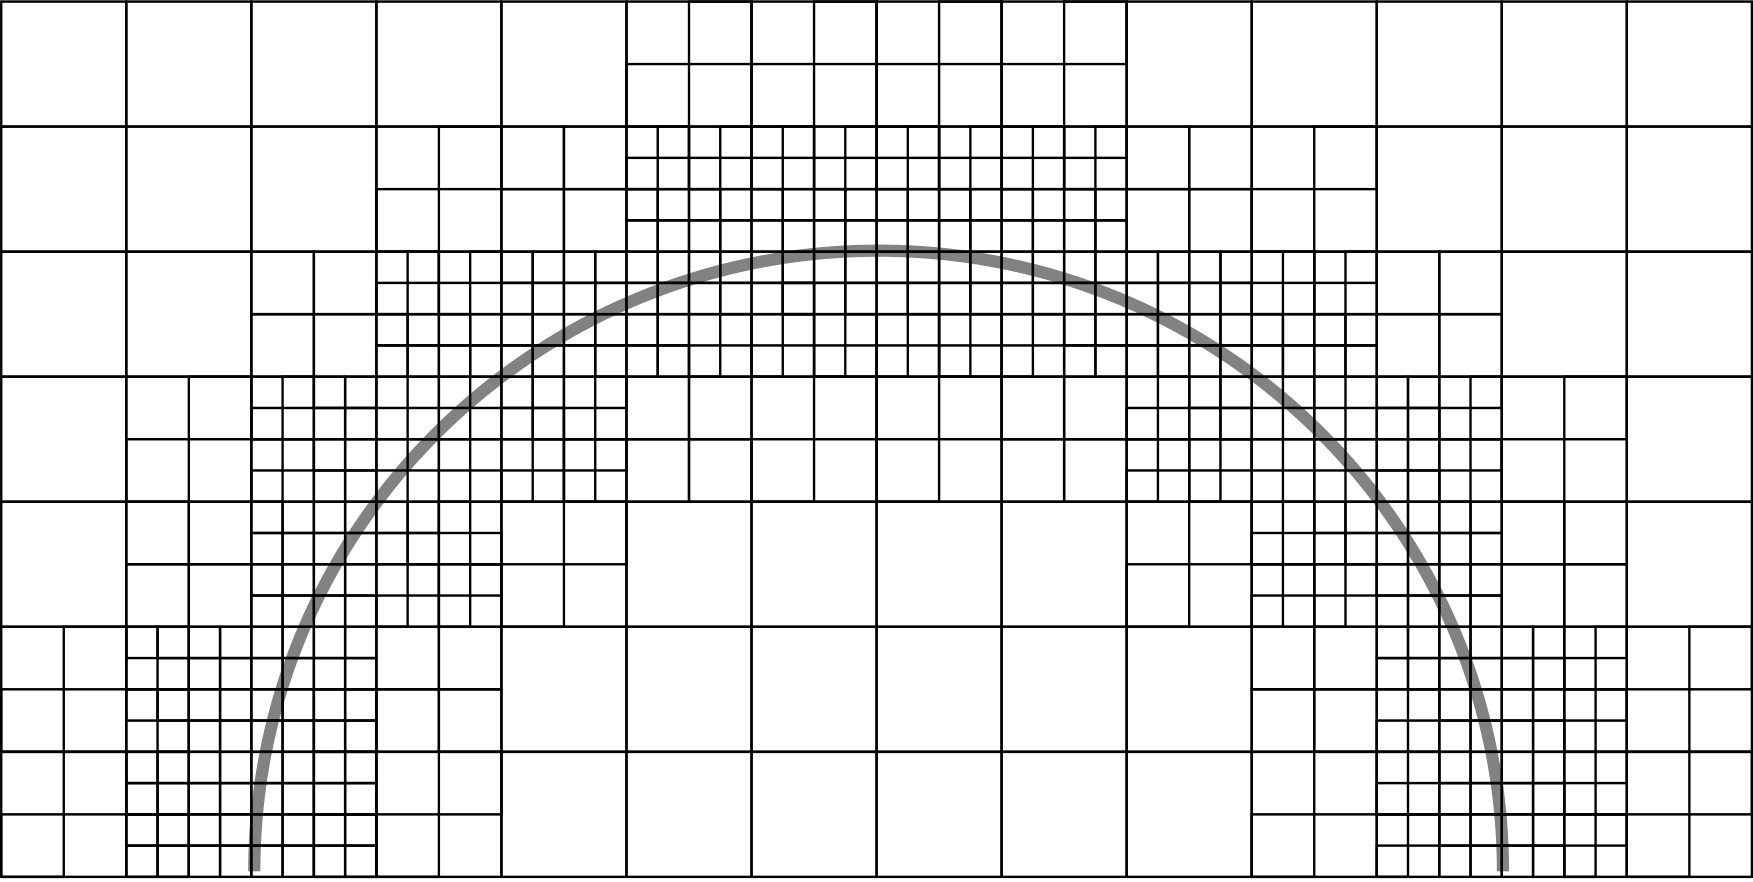
\includegraphics[width=0.5\textwidth,height=0.5\textheight]{block_amr.png}
\caption{AMR Quadtree {[}4{]}}
\end{figure}
\end{frame}

\begin{frame}{yt}
\protect\hypertarget{yt}{}
\begin{itemize}
\tightlist
\item
  yt: Python analysis and visualization package {[}2{]}
\item
  For any type of volumetric data

  \begin{itemize}
  \tightlist
  \item
    Both Enzo and Enzo-E
  \end{itemize}
\end{itemize}
\end{frame}

\begin{frame}
\begin{columns}[T]
\begin{column}{0.5\textwidth}
\begin{figure}
\centering
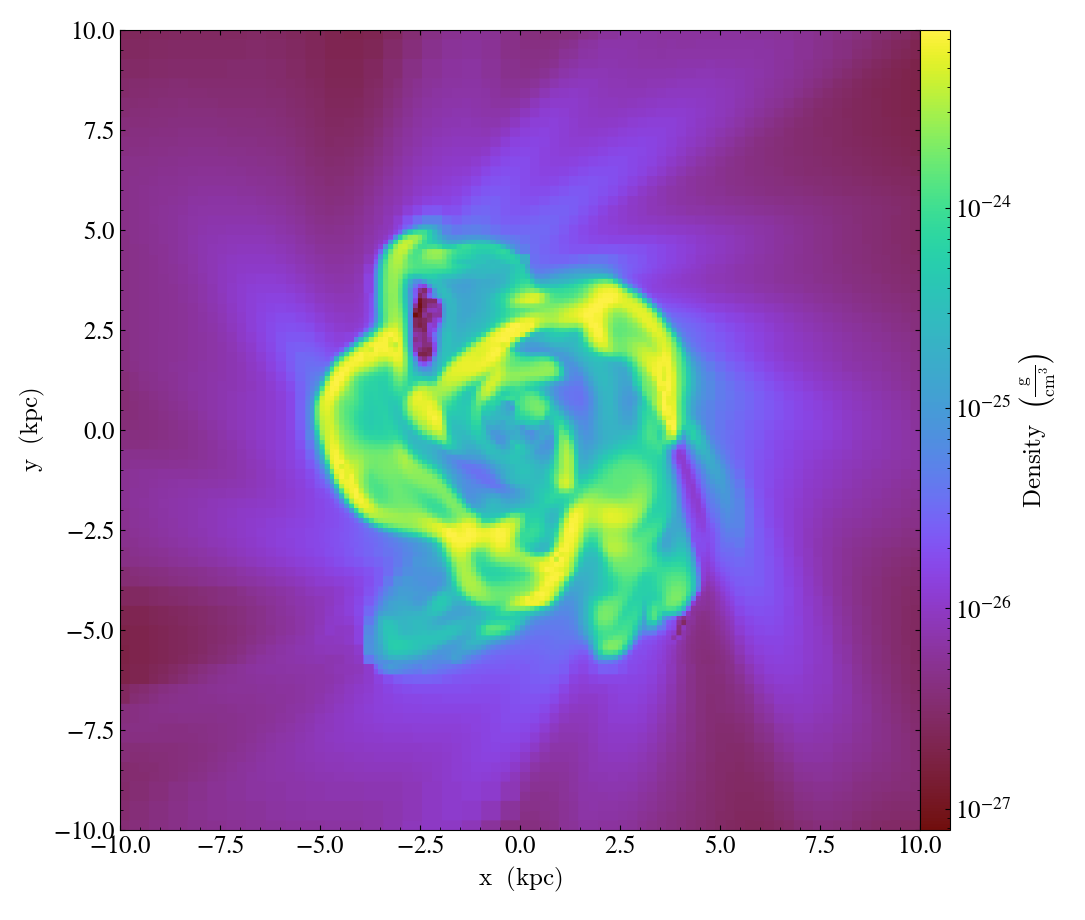
\includegraphics{galaxy0030_Slice_z_density.png}
\caption{Slice over z axis of density}
\end{figure}
\end{column}

\begin{column}{0.5\textwidth}
\begin{figure}
\centering
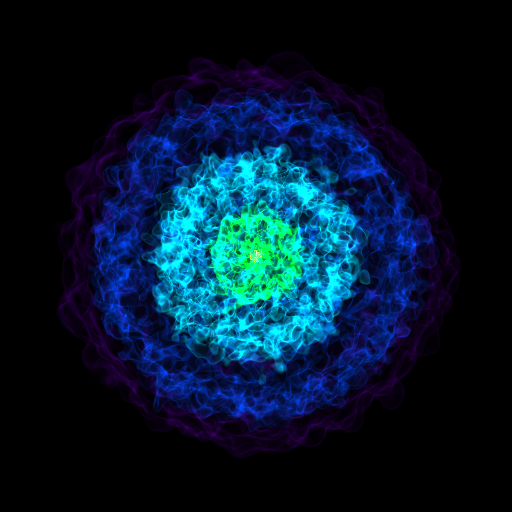
\includegraphics[width=0.85\textwidth,height=0.85\textheight]{galaxy0030_3dviz.png}
\caption{3D visualization of density}
\end{figure}
\end{column}
\end{columns}
\end{frame}

\begin{frame}{Frontends}
\protect\hypertarget{frontends}{}
\begin{itemize}
\tightlist
\item
  yt supports a variety of \textbf{frontends} to load data
\item
  Frontends can be implement in various formats

  \begin{itemize}
  \tightlist
  \item
    Grid-based

    \begin{itemize}
    \tightlist
    \item
      Inconsistent across the domain
    \end{itemize}
  \item
    Array-of-octree
  \end{itemize}
\end{itemize}
\end{frame}

\begin{frame}{Problem}
\protect\hypertarget{problem}{}
Enzo-E analysis in yt is slow!
\end{frame}

\begin{frame}{Problem}
\protect\hypertarget{problem-1}{}
\begin{itemize}
\tightlist
\item
  Slow on large datasets
\item
  Can't practically analyze enzo-e datasets of over \(256^3\) blocks

  \begin{itemize}
  \tightlist
  \item
    \(256^3\) blocks → multiple hours to load in the data
  \end{itemize}
\item
  Needs to analyze datasets of size \(2048^3\) blocks

  \begin{itemize}
  \tightlist
  \item
    \(\approx 1\) TB
  \end{itemize}
\end{itemize}
\end{frame}

\begin{frame}{Current Frontend}
\protect\hypertarget{current-frontend}{}
\begin{itemize}
\tightlist
\item
  Collection of grids

  \begin{itemize}
  \tightlist
  \item
    Each grid is a python object

    \begin{itemize}
    \tightlist
    \item
      \(\approx 1\) KB
    \end{itemize}
  \end{itemize}
\item
  Largely single threaded
\end{itemize}
\end{frame}

\begin{frame}{New frontend}
\protect\hypertarget{new-frontend}{}
\begin{itemize}
\tightlist
\item
  Array of Octree
\item
  Multithreaded
\item
  Each Oct is a C struct

  \begin{itemize}
  \tightlist
  \item
    At most 88 bytes
  \end{itemize}
\end{itemize}
\end{frame}

\begin{frame}{Result}
\protect\hypertarget{result}{}
\begin{itemize}
\tightlist
\item
  Faster
\item
  Can analyze datasets of size \(2048^3\) blocks

  \begin{itemize}
  \tightlist
  \item
    \(\approx 1\) TB
  \end{itemize}
\end{itemize}
\end{frame}

\begin{frame}{Current Status}
\protect\hypertarget{current-status}{}
\begin{itemize}
\tightlist
\item
  New frontend is partially built
\item
  Non refined data can be loaded in
\end{itemize}

\begin{figure}
\centering
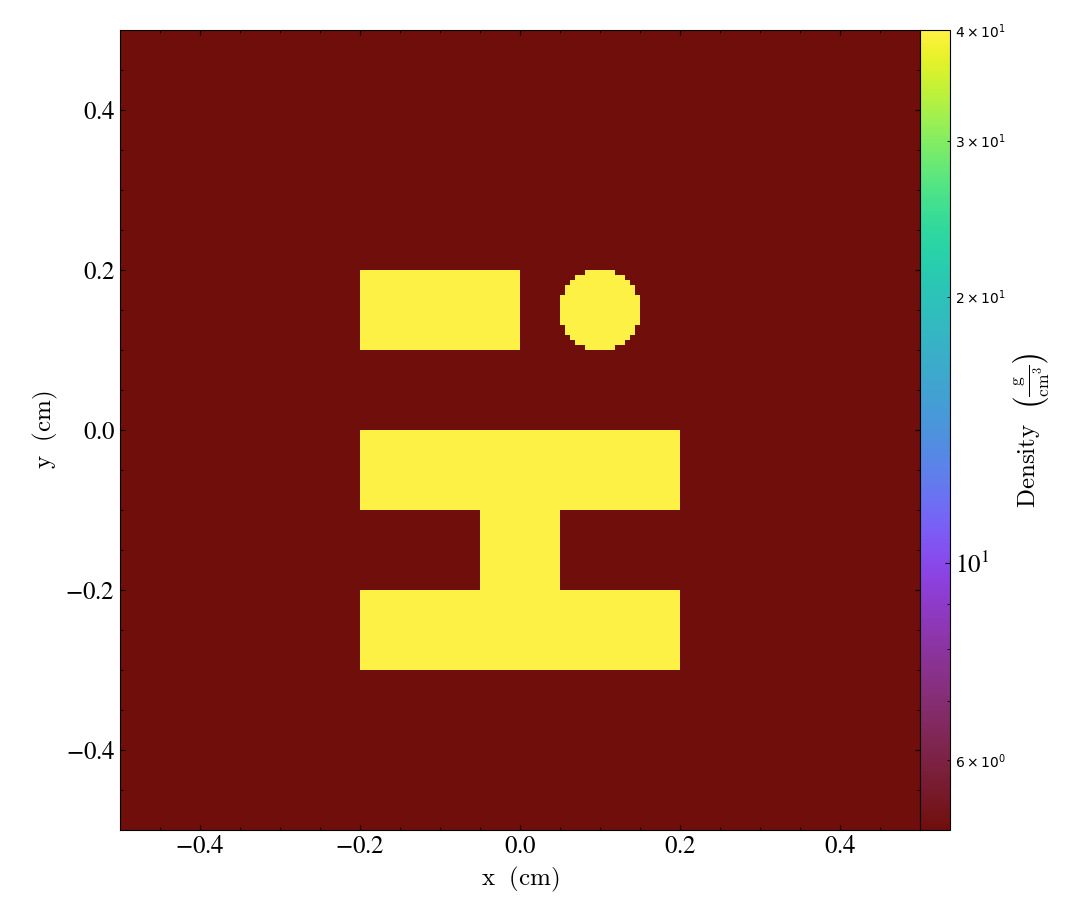
\includegraphics[width=0.5\textwidth,height=0.5\textheight]{new2.jpg}
\caption{Incorrect visualization. The ``Hi'' is mirrored and rotated
from what it should be.}
\end{figure}
\end{frame}

\begin{frame}{Future Work}
\protect\hypertarget{future-work}{}
\begin{itemize}
\tightlist
\item
  New frontend is unoptimized

  \begin{itemize}
  \tightlist
  \item
    Initially slower
  \end{itemize}
\item
  Other simulation codes interpreted as grid-based, instead of oct-based
\end{itemize}
\end{frame}

\begin{frame}[allowframebreaks]{References}
\protect\hypertarget{references}{}
\hypertarget{refs}{}
\begin{CSLReferences}{0}{0}
\leavevmode\vadjust pre{\hypertarget{ref-Bryan_2014}{}}%
\CSLLeftMargin{1. }%
\CSLRightInline{\textbf{{ENZO}: {AN} {ADAPTIVE} {MESH} {REFINEMENT}
{CODE} {FOR} {ASTROPHYSICS}}
\CSLBlock{Greg L Bryan, Michael L Norman, Brian W OShea, Tom Abel, John
H Wise, Matthew J Turk, Daniel R Reynolds, David C Collins, Peng Wang,
Samuel W Skillman, \ldots{} Yuan Li and} \emph{The Astrophysical Journal
Supplement Series} (2014-03)
\url{https://doi.org/10.1088\%2F0067-0049\%2F211\%2F2\%2F19}
\CSLBlock{DOI:
\href{https://doi.org/10.1088/0067-0049/211/2/19}{10.1088/0067-0049/211/2/19}}}

\leavevmode\vadjust pre{\hypertarget{ref-turk}{}}%
\CSLLeftMargin{2. }%
\CSLRightInline{\textbf{{yt: A Multi-code Analysis Toolkit for
Astrophysical Simulation Data}}
\CSLBlock{Matthew J Turk, Britton D Smith, Jeffrey S Oishi, Stephen
Skory, Samuel W Skillman, Tom Abel, Michael L Norman} (2011-01)
\url{https://arxiv.org/abs/1011.3514}
\CSLBlock{DOI:
\href{https://doi.org/10.1088/0067-0049/192/1/9}{10.1088/0067-0049/192/1/9}}}

\leavevmode\vadjust pre{\hypertarget{ref-bordner2018}{}}%
\CSLLeftMargin{3. }%
\CSLRightInline{\textbf{Computational cosmology and astrophysics on
adaptive meshes using charm++}
\CSLBlock{James Bordner, Michael L Norman} (2018)
\url{https://arxiv.org/abs/1810.01319}}

\leavevmode\vadjust pre{\hypertarget{ref-dunning2020}{}}%
\CSLLeftMargin{4. }%
\CSLRightInline{\textbf{Adaptive mesh refinement in the fast lane}
\CSLBlock{D Dunning, W Marts, RW Robey, P Bridges} \emph{Journal of
Computational Physics} (2020)
\url{https://www.sciencedirect.com/science/article/pii/S0021999119308988}
\CSLBlock{DOI: \url{https://doi.org/10.1016/j.jcp.2019.109193}}}

\end{CSLReferences}
\end{frame}

\end{document}
